% Template for PLoS
% Version 3.5 March 2018
%
% % % % % % % % % % % % % % % % % % % % % %
%
% -- IMPORTANT NOTE
%
% This template contains comments intended
% to minimize problems and delays during our production
% process. Please follow the template instructions
% whenever possible.
%
% % % % % % % % % % % % % % % % % % % % % % %
%
% Once your paper is accepted for publication,
% PLEASE REMOVE ALL TRACKED CHANGES in this file
% and leave only the final text of your manuscript.
% PLOS recommends the use of latexdiff to track changes during review, as this will help to maintain a clean tex file.
% Visit https://www.ctan.org/pkg/latexdiff?lang=en for info or contact us at latex@plos.org.
%
%
% There are no restrictions on package use within the LaTeX files except that
% no packages listed in the template may be deleted.
%
% Please do not include colors or graphics in the text.
%
% The manuscript LaTeX source should be contained within a single file (do not use \input, \externaldocument, or similar commands).
%
% % % % % % % % % % % % % % % % % % % % % % %
%
% -- FIGURES AND TABLES
%
% Please include tables/figure captions directly after the paragraph where they are first cited in the text.
%
% DO NOT INCLUDE GRAPHICS IN YOUR MANUSCRIPT
% - Figures should be uploaded separately from your manuscript file.
% - Figures generated using LaTeX should be extracted and removed from the PDF before submission.
% - Figures containing multiple panels/subfigures must be combined into one image file before submission.
% For figure citations, please use "Fig" instead of "Figure".
% See http://journals.plos.org/plosone/s/figures for PLOS figure guidelines.
%
% Tables should be cell-based and may not contain:
% - spacing/line breaks within cells to alter layout or alignment
% - do not nest tabular environments (no tabular environments within tabular environments)
% - no graphics or colored text (cell background color/shading OK)
% See http://journals.plos.org/plosone/s/tables for table guidelines.
%
% For tables that exceed the width of the text column, use the adjustwidth environment as illustrated in the example table in text below.
%
% % % % % % % % % % % % % % % % % % % % % % % %
%
% -- EQUATIONS, MATH SYMBOLS, SUBSCRIPTS, AND SUPERSCRIPTS
%
% IMPORTANT
% Below are a few tips to help format your equations and other special characters according to our specifications. For more tips to help reduce the possibility of formatting errors during conversion, please see our LaTeX guidelines at http://journals.plos.org/plosone/s/latex
%
% For inline equations, please be sure to include all portions of an equation in the math environment.
%
% Do not include text that is not math in the math environment.
%
% Please add line breaks to long display equations when possible in order to fit size of the column.
%
% For inline equations, please do not include punctuation (commas, etc) within the math environment unless this is part of the equation.
%
% When adding superscript or subscripts outside of brackets/braces, please group using {}.
%
% Do not use \cal for caligraphic font.  Instead, use \mathcal{}
%
% % % % % % % % % % % % % % % % % % % % % % % %
%
% Please contact latex@plos.org with any questions.
%
% % % % % % % % % % % % % % % % % % % % % % % %

\documentclass[10pt,letterpaper]{article}
\usepackage[top=0.85in,left=2.75in,footskip=0.75in]{geometry}

% amsmath and amssymb packages, useful for mathematical formulas and symbols
\usepackage{amsmath,amssymb}

% Use adjustwidth environment to exceed column width (see example table in text)
\usepackage{changepage}

% Use Unicode characters when possible
\usepackage[utf8x]{inputenc}

% textcomp package and marvosym package for additional characters
\usepackage{textcomp,marvosym}

% cite package, to clean up citations in the main text. Do not remove.
% \usepackage{cite}

% Use nameref to cite supporting information files (see Supporting Information section for more info)
\usepackage{nameref,hyperref}

% line numbers
\usepackage[right]{lineno}

% ligatures disabled
\usepackage{microtype}
\DisableLigatures[f]{encoding = *, family = * }

% color can be used to apply background shading to table cells only
\usepackage[table]{xcolor}

% array package and thick rules for tables
\usepackage{array}

% create "+" rule type for thick vertical lines
\newcolumntype{+}{!{\vrule width 2pt}}

% create \thickcline for thick horizontal lines of variable length
\newlength\savedwidth
\newcommand\thickcline[1]{%
  \noalign{\global\savedwidth\arrayrulewidth\global\arrayrulewidth 2pt}%
  \cline{#1}%
  \noalign{\vskip\arrayrulewidth}%
  \noalign{\global\arrayrulewidth\savedwidth}%
}

% \thickhline command for thick horizontal lines that span the table
\newcommand\thickhline{\noalign{\global\savedwidth\arrayrulewidth\global\arrayrulewidth 2pt}%
\hline
\noalign{\global\arrayrulewidth\savedwidth}}


% Remove comment for double spacing
%\usepackage{setspace}
%\doublespacing

% Text layout
\raggedright
\setlength{\parindent}{0.5cm}
\textwidth 5.25in
\textheight 8.75in

% Bold the 'Figure #' in the caption and separate it from the title/caption with a period
% Captions will be left justified
\usepackage[aboveskip=1pt,labelfont=bf,labelsep=period,justification=raggedright,singlelinecheck=off]{caption}
\renewcommand{\figurename}{Fig}

% Use the PLoS provided BiBTeX style
% \bibliographystyle{plos2015}

% Remove brackets from numbering in List of References
\makeatletter
\renewcommand{\@biblabel}[1]{\quad#1.}
\makeatother



% Header and Footer with logo
\usepackage{lastpage,fancyhdr,graphicx}
\usepackage{epstopdf}
%\pagestyle{myheadings}
\pagestyle{fancy}
\fancyhf{}
%\setlength{\headheight}{27.023pt}
%\lhead{
\includegraphics[width=2.0in]{PLOS-submission.eps}}
\rfoot{\thepage/\pageref{LastPage}}
\renewcommand{\headrulewidth}{0pt}
\renewcommand{\footrule}{\hrule height 2pt \vspace{2mm}}
\fancyheadoffset[L]{2.25in}
\fancyfootoffset[L]{2.25in}
\lfoot{\today}

%% Include all macros below

\newcommand{\lorem}{{\bf LOREM}}
\newcommand{\ipsum}{{\bf IPSUM}}


% tightlist command for lists without linebreak
\providecommand{\tightlist}{%
  \setlength{\itemsep}{0pt}\setlength{\parskip}{0pt}}

% From pandoc table feature
\usepackage{longtable,booktabs,array}
\usepackage{calc} % for calculating minipage widths
% Correct order of tables after \paragraph or \subparagraph
\usepackage{etoolbox}
\makeatletter
\patchcmd\longtable{\par}{\if@noskipsec\mbox{}\fi\par}{}{}
\makeatother
% Allow footnotes in longtable head/foot
\IfFileExists{footnotehyper.sty}{\usepackage{footnotehyper}}{\usepackage{footnote}}
\makesavenoteenv{longtable}

% Pandoc citation processing
\newlength{\cslhangindent}
\setlength{\cslhangindent}{1.5em}
\newlength{\csllabelwidth}
\setlength{\csllabelwidth}{3em}
\newlength{\cslentryspacingunit} % times entry-spacing
\setlength{\cslentryspacingunit}{\parskip}
% for Pandoc 2.8 to 2.10.1
\newenvironment{cslreferences}%
  {}%
  {\par}
% For Pandoc 2.11+
\newenvironment{CSLReferences}[2] % #1 hanging-ident, #2 entry spacing
 {% don't indent paragraphs
  \setlength{\parindent}{0pt}
  % turn on hanging indent if param 1 is 1
  \ifodd #1
  \let\oldpar\par
  \def\par{\hangindent=\cslhangindent\oldpar}
  \fi
  % set entry spacing
  \setlength{\parskip}{#2\cslentryspacingunit}
 }%
 {}
\usepackage{calc}
\newcommand{\CSLBlock}[1]{#1\hfill\break}
\newcommand{\CSLLeftMargin}[1]{\parbox[t]{\csllabelwidth}{#1}}
\newcommand{\CSLRightInline}[1]{\parbox[t]{\linewidth - \csllabelwidth}{#1}\break}
\newcommand{\CSLIndent}[1]{\hspace{\cslhangindent}#1}

\usepackage{float}
\usepackage{booktabs}
\newcommand{\beginsupplement}{ \setcounter{table}{0}     \renewcommand{\thetable}{S\arabic{table}}\setcounter{figure}{0} \renewcommand{\thefigure}{S\arabic{figure}}}



\usepackage{forarray}
\usepackage{xstring}
\newcommand{\getIndex}[2]{
  \ForEach{,}{\IfEq{#1}{\thislevelitem}{\number\thislevelcount\ExitForEach}{}}{#2}
}

\setcounter{secnumdepth}{0}

\newcommand{\getAff}[1]{
  \getIndex{#1}{a,b}
}

\begin{document}
\vspace*{0.2in}


% Title must be 250 characters or less.
\begin{flushleft}
{\Large
\textbf\newline{Field and experimental data together with computational
models reveal how cleaner fish adjust decisions in a biological
market} % Please use "sentence case" for title and headings (capitalize only the first word in a title (or heading), the first word in a subtitle (or subheading), and any proper nouns).
}
\newline
% Insert author names, affiliations and corresponding author email (do not include titles, positions, or degrees).
\\
Andrés E. Quiñones\textsuperscript{\getAff{a}}\textsuperscript{*},
Zegni Triki\textsuperscript{\getAff{b}},
Redouan Bshary\textsuperscript{\getAff{Institute of Biology, University
of Neuchatel}}\\
\bigskip
\textbf{\getAff{a}}Institute of Biology,University of Neuchatel ,Rue
Emile-Argand 11, 2000-CH Neuchatel, Switzerland\\
\textbf{\getAff{b}}Department of Zoology, Stockholm University, Svante
Arrheniusväg 18 B, 106 91 Stockholm, Sweden,\\
\bigskip
* Corresponding author: andresqp@gmail.com\\
\end{flushleft}
% Please keep the abstract below 300 words
\section*{Abstract}
While it is generally straightforward to quantify individual performance
in cognitive experiments, identifying the underlying cognitive processes
remains a major challenge. Often, different mechanistic underpinnings
yield similar performances, and Lloyd Morgan's cannon warrants
acceptance of the simpler explanation. Alternatively, when the different
mechanisms interact with environmental conditions, variation in
performance across environments might allow to statistically infer the
mechanism responsible. We illustrate this point by fitting computational
models to experimental data on performance by wild-caught cleaner fish
\emph{Labroides dimidiatus} in an ephemeral reward task, as well as
cleaner and client fish densities from the locations of capture. Using
Bayesian statistics to fit the model parameters to performance data
revealed that cleaner fish most likely estimate future consequences of
an action, while it appears unlikely that the removal of the ephemeral
reward acts as psychological punishment (negative reinforcement).
Incorporating future consequences also yields performances that can be
considered the result of locally optimal decision-rules, in contrast to
the negative reinforcement mechanism. We argue that the combination of
computational models with data is a powerful tool to infer the
mechanistic underpinnings of cognitive performance.

% Please keep the Author Summary between 150 and 200 words
% Use first person. PLOS ONE authors please skip this step.
% Author Summary not valid for PLOS ONE submissions.
\section*{Author summary}
Performance in behavioural experiments is often used to assess the
cognitive abilities of animals. However, animals can get to the same
outcome in alternative ways. Thus, the outcome of the experiments does
not tell us how animals achieve their performance. In order to overcome
this limitation, we used a set of computational models, which provide
predictions on how alternative cognitive mechanisms perform in the face
of varying environmental conditions, and compare their predictions to
performance data from individuals that experienced different conditions
throughout their life. Our study system is the cleaner fish
\emph{Labroides dimidiatus}, a coral reef fish that feeds off
ectoparasites and dead tissue from the skin of other reef fishes.
Cleaner fish often have to choose among alternative clients seeking
their cleaning service, and the optimal choice is often hard to achieve.
Our performance experiments mimic the natural choices the cleaner fish
make. The combination of experiments and computational models points to
cleaner fish abilities to account for the future effect of their choices
by estimating the long term expected value of those choices. Estimating
long term value is a mechanism involved in human foresight.

\linenumbers

% Use "Eq" instead of "Equation" for equation citations.
\emph{Text based on plos sample manuscript, see
\url{https://journals.plos.org/ploscompbiol/s/latex}}

\hypertarget{introduction}{%
\subsection{Introduction}\label{introduction}}

Often alternative cognitive mechanisms yield similar behaviour and/or
cognitive performances. This poses a problem for disentangling the
mechanistic underpinnings of behaviour. This is particularly clear in
research aimed at discovering between species variation in \emph{higher}
cognitive abilities; or in other words, research on whether non-human
animals show cognitive abilities believed to be uniquely human. For
instance, when researchers try to find \emph{mental time travel-like}
behaviour, they usually come up with clever experiments to show the
behaviour displayed requires inferences made through past events{[}1{]}.
However, they often face the challenge of alternative scenarios where
simpler explanations, like classic associative learning, can bring about
the observed behavioural outcome {[}2{]}. Similarly, attempts to
demonstrate the presence of \emph{theory of mind} in non-human animals
face objections justified by alternative mechanisms underpinning similar
behavioural results {[}3{]}. Such controversies are usually settled by
using the principle of parsimony and its cognitive version, Lloyd
Morgan's cannon, which states that the simpler explanation (mechanism)
should be accepted. Ideally, however, alternative hypotheses should be
evaluated in light of their explanatory power. One potential dimension
that could allow the variation necessary among distinct cognitive
mechanisms is environmental variation. Controlled laboratory conditions
often mask between and within species variation that arises among
different environments. Thus, if predictions from the alternative
mechanisms depend on environmental conditions, it is possible to assess
their relative explanatory power by performing cognitive test in the
context of different environmental conditions.

From an evolutionary perspective, mechanisms are likely selected because
of how they allow individuals to respond to environmental variation. For
example, biological market theory predicts that the exchange rate of
goods and/or services traded between cooperative partners adjusts to the
law of supply and demand, when individuals have some degree of partner
choice {[}4{]}. Supply and demand conditions, which typically depend on
the abundance of the species involved, certainly vary in time and space.
Therefore, natural selection should favour the ability to flexibly
adjust decisions and behavioural output to current market conditions.
Indeed, such adjustments have been repeatedly documented {[}5{]}. In
animals, an obvious general candidate mechanism for the strategic
adjustment is the cognitive machinery. However, it is not clear which
cognitive mechanisms allow individuals to adjust their behaviour to the
varying conditions. More specifically the question arises to what extent
mechanisms beyond basic associative learning may be involved.

One example of strategic adjustment in a biological market is the marine
cleaning mutualism involving the cleaner fish \emph{Labroides
dimidiatus} and `client' fish. Client fish seek cleaner fish services at
their territory (so-called ``cleaning station'') and offer themselves as
food patches to get their ectoparasites removed, which provides cleaners
with food and clients with improved health {[}6--9{]}. Given the
capacity of some client fish to swim larger distances and access
multiple cleaning stations while others access the only cleaning station
in their territory, it is crucial to categorize clients as either
``visitors'' or ``residents,'' respectively. During cleaning
interactions, a cleaner fish often face a choice between a visitor and a
resident client seeking its cleaning services simultaneously. Visitors
have the option to switch to another cleaner fish if being made to wait,
while residents must wait for inspection. Indeed, visitors have been
observed to use their partner choice option in that way {[}10{]}, which
may explain why cleaners give visitors service priority in a field study
in the Red Sea {[}11{]}.

When researchers aimed at testing wild-caught cleaner fish, as well as
individuals from other species, abilities to prioritize visitor over
resident clients in a lab-based paradigm, they used Plexiglas plates of
different colours and shapes offering the same amount of food as
surrogates for visitor and resident clients. One plate is made to behave
like a resident, i.e.~it remains until the cleaner fish has eaten off
it. The other plate was made to behave like a visitor, i.e.~it is
removed if not inspected first. This laboratory paradigm originally
inspired by the cleaning market of cleaner fish is more generally
referred as the ephemeral reward task. Individuals are assessed in their
capacity to develop a preference for the ephemeral option, which gives
them access to two reward units. Cleaners learned to prefer the visitor
plate and hence obtained the double amount of food {[}12{]}.
Furthermore, adult cleaner fish outperformed various primates as well as
rats and pigeons in this original version of the ephemeral reward task
{[}13,14{]}; yet the African grey parrots solve this task as well
{[}15{]}. This between variation in performance, and primates' known
cognitive abilities {[}\textbf{reader\_Evolution\_2001?}{]}, shows that
performance in the task cannot be readily explained by classifying
species as having high and low cognitive abilities. Instead, this
between species variation suggests that solving the ephemeral reward
task requires a set of cognitive mechanisms that are not present in all
the tested taxa, or were not used under the experimental set-up.

Recent research on the cognitive abilities needed to solve the ephemeral
reward task has used a broad approach as proposed by Shettleworth
{[}16{]}, who defined cognition as including all ways in which animals
acquire information through the senses, process, retain and decide to
act on it. Indeed, perception of relevant cues is of major importance
for individual performance. For example, some animals find relevant
information in the plates {[}17{]} while others find it in the food
{[}18,19{]}. However, identifying cues as salient is not the only
challenge of the ephemeral reward task, as revealed by proximate
learning models. Such models allow varying the cognitive tool kit and
evaluating which minimal kit is necessary to solve the task at hand
(e.g. {[}20{]}). Applied to the ephemeral reward task, learning models
showed that basic reinforcement learning does not suffice to solve the
ephemeral reward task {[}21,22{]}. This is particularly so when models
assume the more complex natural situation in which cleaner fish face not
only resident-visitor pairs but also visitor-visitor and
resident-resident pairs, as well a resident alone or a visitor alone. To
be able to give visitors priority over residents, cleaners need to be
able to assess a client's value separately for the three possible
scenarios (alone, paired with a fish with the same strategic option,
paired with a fish with the alternative strategic option) {[}22{]}. The
ability to distinguish and value one stimulus differently alone from
compound versions of it has been termed configurational learning,
chunking, or segmentation (see references in {[}21{]}).

In addition to configurational learning, cleaners also need to account
for the future consequences of current decisions. In the model by
Quiñones \emph{et al.} {[}22{]}, this could be achieved in two
non-mutually exclusive ways: through low temporal discounting of future
effects, also termed `chaining' {[}23{]}; and/or through perceiving a
visitor client leaving as psychological punishment (i.e.~as a negative
reinforcer). Low temporal discounting is when individuals include in
their valuation of an action the reward effects that this will have in
the future. This is done by combining in a single valuation the reward
obtained in the current time with all the reward that comes after,
discounting for how far in the future reward is accrued. `Chaining' the
reward of these different time steps allows individuals to take actions
that increase the long-term reward at the sacrifice of short term
considerations {[}23{]}. Even though, `chaining' can be readily
implemented computationally in learning models {[}23,24{]}, cognitively
it seems to be a complex adaptation {[}2{]}. On the other hand, using
client behaviour as a negative reinforcer is, in principle, easier to
implement. Negative reinforcement is part of the ubiquitous learning
mechanism termed operant conditioning {[}25,26{]}. Thus, the standard
logic of Lloyd Morgan's cannon demands that operant conditioning as the
simpler explanation is to be accepted by default. Ideally, however, the
two mechanisms should be evaluated in light of how well they explain the
available data. Note that different fields interested in cognition and
decision making use different words to refer to negative reinforcers
{[}22,24{]}. Here, for the sake of simplicity and clarity, we will use
the word `penalty' to refer to this mechanism which includes a negative
reinforcer.

Over the last decade, our team tested over a hundred wild-caught cleaner
fish in the exact same paradigm of the ephemeral reward task
{[}13,27--30{]}. These fish often come from different reef locations
around the study field site at Lizard Island, Great Barrier Reef in
Australia. Further investigation of the local eco-sociological
conditions revealed that cleaner and client fish population densities
have a substantial impact on cleaner fish performance in the task.
Cleaner fish from reef sites with relatively low densities were more
likely to fail at solving the task {[}27--29{]}. The explanation for
this pattern is twofold. First, low cleaner fish population densities
imply low supply and high demand for cleaning services. Under such
conditions, there are fewer occasions under which failing to give
priority to a visitor translates to an empty cleaning station. Second
and also related to the state of the cleaning market, visitor clients at
low cleaner fish population densities are less likely to exert their
partner choice options and are hence more likely to wait for inspection
if not given cleaning priority {[}30{]}. In the absence of partner
choice cleaner fish should not give priority to visitors any more.

The interplay between the underlying cognitive machinery and local
ecological conditions apparently generate the documented variable
performance among individuals of the same species. Our approach of
fitting the computational model to the empirical data on fish densities
and cleaner fish censuses and performance in the ephemeral reward task
aimed at: (i), determining which mechanism cleaner fish use to
incorporate future consequences of current decisions by testing whether
chaining, penalty, or a combination of both best explains their
performance; (ii) determining whether the two mechanisms differed with
respect to the ecological conditions that are likely to cause high
versus low performance in the ephemeral reward task. Additionally, we
assessed which mechanism yields optimal performance patterns. Relying on
the logic of biological market theory, we predicted that appropriate
performance is to show a low preference for visitors under low local
cleaner-to-client ratio.

\hypertarget{methods}{%
\subsection{Methods}\label{methods}}

\hypertarget{the-model}{%
\subsubsection{The model}\label{the-model}}

The model consists of a set of individual-based simulations where
individuals, representing cleaner fish, face a series of choices between
two options, which simulate the natural conditions of the cleaning
market. Individuals experience a series of discrete time points in which
they face different `states,' defined by the number and category of
client fish (visitor or residents) inviting for cleaning services. There
are six possible states: zero clients, one resident, one visitor,
resident-resident, visitor-visitor, and resident-visitor. The
probability of each state is largely determined by the relative
abundance of cleaner fish, residents and visitors, but to some degree by
cleaner fish choices when it faces the resident-visitor combination.
This is because residents are willing to queue for cleaning service;
while visitors leave the queue (with a certain probability) when made to
wait. Individuals obtain a fixed reward from cleaning a client fish
regardless of the category. Every time individuals face and make a
choice they update the probability of making that same choice. The
update is based on the difference between the expected reward and the
obtained reward (prediction error) {[}24,31{]}. Given the new
information, the update is carried in the direction that leads to more
reward being obtained, given the new information. In the long run, the
probability of choosing a visitor over a resident converges in the
model. To which probability the model will converge depends on the
relative abundance of cleaners, visitors and residents; as well as on
the probability of visitors leaving the cleaning station when made to
wait. Further details of the model implementation can be found in
Quiñones \emph{et al} {[}22{]}.

The model shows that agents need to find a way to incorporate future
consequences of current choices. In the model, this could be achieved
with either of two parameters that could also work together. First,
\(\gamma\) measures how much individuals include future rewards in their
decision updates. If \(\gamma=0\), individuals only use the immediate
reward obtained from a cleaning interaction. As \(\gamma\) increases,
individuals include more the reward obtained from the subsequent
choices. That amounts to calculating and using for decision making the
future expected rewards of an action (chaining). Second, \(\eta\)
measures how much individuals include in their reward the fleeing
behaviour of visitors as a negative component (penalty). Both of these
parameters allow individuals to use in their estimates the future
effects of their choices.

\hypertarget{empirical-data}{%
\subsubsection{Empirical data}\label{empirical-data}}

The empirical data were collected between 2010 and 2019 always during
the austral winter months June to August from a total of five study reef
sites (Corner Beach-CB, Horseshoe-HS, Mermaid Cove-MC, Northern
Horseshoe-NHS, and The Crest-TC) at Lizard Island
(\(14.6682^\circ S, 145.4604^\circ E\)), Great Barrier Reef, Australia.
The data consist of three sets: fish censuses, field observations of
cleaner-client interactions to quantify the probability of visitors
leaving if made to wait, and the performance of wild-caught cleaner fish
in the ephemeral reward test. In total, we have twelve site/year data
sets for fish censuses and corresponding performance in the lab test.
Thus, some sites were sampled more than once. To estimate the population
density of cleaner fish and their clients at a given site in a given
year, Triki \emph{et al.} {[}29{]} used a series of ten transects of
\(30m\) each. Observers swam along the transect lines placed on the reef
and first counted the visible large-bodied adult fish (species with
total length \(TL \geq 10cm\)) including cleaner fish on a width of
\(5m\), and then on the return individuals of small-bodied fish species
(\(TL < 10 cm\))\\
on a width of \(1 m\) (see Triki et al.~2018 for further details on fish
censuses data collection). We then scaled the counts of cleaner fish,
small-bodied, and large-bodied clients fish densities per \(100 m^2\).
From the study by Triki \emph{et al} {[}29{]} cleaner fish and
large-bodied client populations densities were highly correlated, and
only the former was hence used in the analyses as representative of both
measures.

The field observation data consisted of video recordings/encodings of
the cleaner-client cleaning interactions. There were videos from eight
cleaners per site/year of a duration of \(30 min\) each. Triki \emph{et
al} extracted information from every event wherein a visitor client was
made to wait in favour of another client (visitor or resident), and
noted whether or not the visitor left or queued for the cleaning service
{[}29,30{]}.

The cognitive performance data was from a total of 120 cleaners (10
individuals per 12 site/year) tested in the ephemeral reward task
{[}29,30{]}. Authors housed all captured cleaners individually in glass
aquaria ( \(62cm \times 27cm \times 37 cm\) ) and provided them with PVC
pipes (\(10 cm \times 1 cm\)) as shelters. The task consisted of
exposing the cleaner fish to substitute models of client fish in the
form of two \emph{Plexiglas} plates offering the same amount of food
(one item of mashed prawn). The two plates differed in colour and
pattern (horizontal green stripes or vertical pink stripes) but had
equal size (\(10 cm \times 7 cm\)). Importantly, the two plates played
different roles as either a visitor (ephemeral food source) or resident
(permanent food source). That is, if a cleaner fish inspected the
resident plate first, the experimenter withdrew the visitor plate out of
the aquarium as a consequence. Choosing first the visitor plate,
however, granted access to both plates. The equal size of the plates
forced cleaner fish to learn to give service priority to the visitor
plate based solely on the behaviour-cue of the plates rather than
size-cue {[}17{]}. Triki \emph{et al.} {[}29,30{]} tested the fish for a
maximum of 200 trials with 20 trials a day, 10 trials in the morning and
10 trials in the afternoon. They randomized and counterbalanced the
plates' spatial location (i.e.~left or right) between trials. Similarly,
they counterbalanced the plates' decoration (colour and pattern) and the
plates' role (visitor or resident) between the tested fish. In the
original studies, once a fish reach a learning criterion, that is,
performing significantly above chance level (\(> 50%
\), \(p-value ≥ 0.05\)), they passed to a reversal version of the task
where the roles of the visitor/resident Plexiglas plates were swapped
(see Triki et al.~2019, 2020). Here, we used instead a subset of these
data in order to have an idea of cleaner fish preferences for the
visitor plate, even if they do not reach the learning criterion within
200 trials. To do so, we first extracted the trial-by-trial outcomes
from the last two sessions (20 trials) of those who never reached the
learning criterion for visitor plate (\(N = 45\) cleaner fish). For
those who reached the learning criterion at some point during the test
and passed to a reversal phase, we extracted the trial-by-trial outcomes
from the last session (10 trials) before passing to reversal and the
last 10 trials they were exposed to in the test (\(N = 75\) cleaner
fish). We chose a combination of initial and reversal to quantify
preference for the visitor client, given that it matches well the
criteria chosen in previous analysis of the ephemeral reward task
experimental set-up {[}29,30{]}. In the supplementary material (Fig.
\ref{fig:rawdata}) we show how our choice maps to the previously used
criteria. For comparison, we also show a quantification of visitor
preference based only on the initial phase of the task.

\hypertarget{statistical-analysis}{%
\subsubsection{Statistical analysis}\label{statistical-analysis}}

The aim of the analyses is to fit the key model parameters \(\gamma\)
and \(\eta\), to the empirical data from Triki \emph{et al.} {[}29,30{]}
to test whether each or a combination of these effects is a better
explanation for the pattern seen in the data. We used the ecological
variables: cleaners, visitor clients, resident clients abundances and
visitor clients leaving probability,\\
as input to the models. As the response variable, we used cleaners'
preference for visitors over residents in the ephemeral reward task.
Finally, we used the preference for visitors resulting from the model
simulations as the prediction for the response variable. We kept all
other parameter values used for the model simulations constant, see
Table \ref{tab:param}.

To capture with the model the relationship between the ecological
variables and cleaner fish preferences for visitors, we needed to scale
the absolute population densities of cleaner fish from the empirical
data to a measure of relative abundances that captures client visitation
patterns. This is because, in the model, relative abundances of clients
define not only the probability of residents and visitors but also how
often the cleaning station is empty (e.g.~there are no clients to be
cleaned). The frequency with which clients visit the station is another
variable, which in nature may vary among different client species
depending on their ectoparasite loads. We do not have field estimates
for species-specific parasite loads, especially not as a function of the
site. In order to control for these aspects, we computed a measure of
relative cleaner fish abundance for each reef site relative to absolute
abundances and multiplied it by a scaling constant that changes the
range of the variable. This scaling constant is hence meant to capture
variation in the market conditions driven partly by cleaner fish
abundance. We fitted the value of the scaling constant as part of the
statistical inference. As for the visitor and resident abundances, we
computed a relative measure with respect to the total client abundance,
and weighted that by the rescaled relative absence of cleaners
(\(1-\text{relative cleaner abundance}\)). Thus, all three measures of
relative abundance sum up to 1, and can be used in the model as a proxy
for the probability of having different options in the cleaning station.
Note that we introduced the scaling constant to control for variation
that is not captured by the model; its parameter distribution does not
offer biological insights.

Once we calculated the relative abundances, we obtained predictions from
the model for each one of the locations and ran the Markov Chain. We
started the chain with random values for the parameters of interest,
then ran the computational model once for every reef site using as input
the ecological explanatory variables. The model outputs the probability
of choosing the visitor for each location \(p_i\), where \(i\) is the
index for the 12 locations. Assuming a binomial distribution, the
probability that each of the cleaner fish 20 choices in the ephemeral
reward task was generated by the model is given by
\(\binom{n}{k_ij}p^{k_{ij}}_i (1-p_i)^{n-k_{ij}}\); where \(k_{ij}\) is
the number of times that cleaner fish \(j\) in reef site \(i\) chose the
visitor over the resident; and \(n=20\) (due to our choice of using 20
choices per cleaner fish). By taking the natural logarithm and summing
over all the cleaner fish and reef sites, we obtained the log-likelihood
of the data given the model and parameters. We then proposed a new set
of parameters drawn from a uniform distribution centred around the old
parameter set. The amplitude of the uniform distribution used for each
parameter can be found in Table \ref{tab:param}. Subsequently, we ran
the model and calculated the likelihood with the new parameter set. We
then used the ratio of the two likelihoods to choose which parameter set
to keep. New parameter sets with a higher likelihood than the old set
replaced old ones, and those with a lower likelihood replaced current
ones with a probability equal to the log-likelihood ratio. Given that we
only used the likelihoods in the decision, we used an uninformative
prior. Once we decided whether the new parameter set would replace the
old one, we ran the model again to sample the likelihood distribution of
the parameter set. We then started the cycle again by proposing a new
set of parameters and repeated the process for \(1e^5\) steps. We ran 5
independent chains, discarded the first \(1000\) samples of each chain
as burn in, and after that, we kept 1 in every 100 samples to avoid
autocorrelation. The collection of parameters sets kept in all chains
approximates the posterior distribution. We coded the model as well as
the fitting algorithm in \emph{c++}, the diagnostics and visualization
in R {[}32{]}. All codes are accessible at
\url{https://github.com/andreseqp/learnDatamodel}

To compare the fit of the three alternative models, we used the
distribution of pseudo \(R^2\) proposed by Mcfadden {[}33{]}. Mcfadden's
pseudo \(R^2\) is a standard measure of fit for logistic regression. In
that context, \(pseudo-R^2\) uses the log-likelihood of the data given
the model, relative to the log-likelihood of the data given a model
without covariates, as a measure of fit. Our model is not a logistic
regression, therefore we measured the \(pseudo-R^2\) in relation to the
log-likelihood of a model with parameters \(\gamma\) and \(\eta\) set to
zero. This, in practice, amounts to a model that has a neutral
preference between the two options. We computed the pseudo \(R^2\) for
all the samples of the posterior from the MCMC. Thus, we used these
distributions of pseudo \(R^2\)'s as a measure of fit.

\hypertarget{results}{%
\subsection{Results}\label{results}}

\begin{figure}
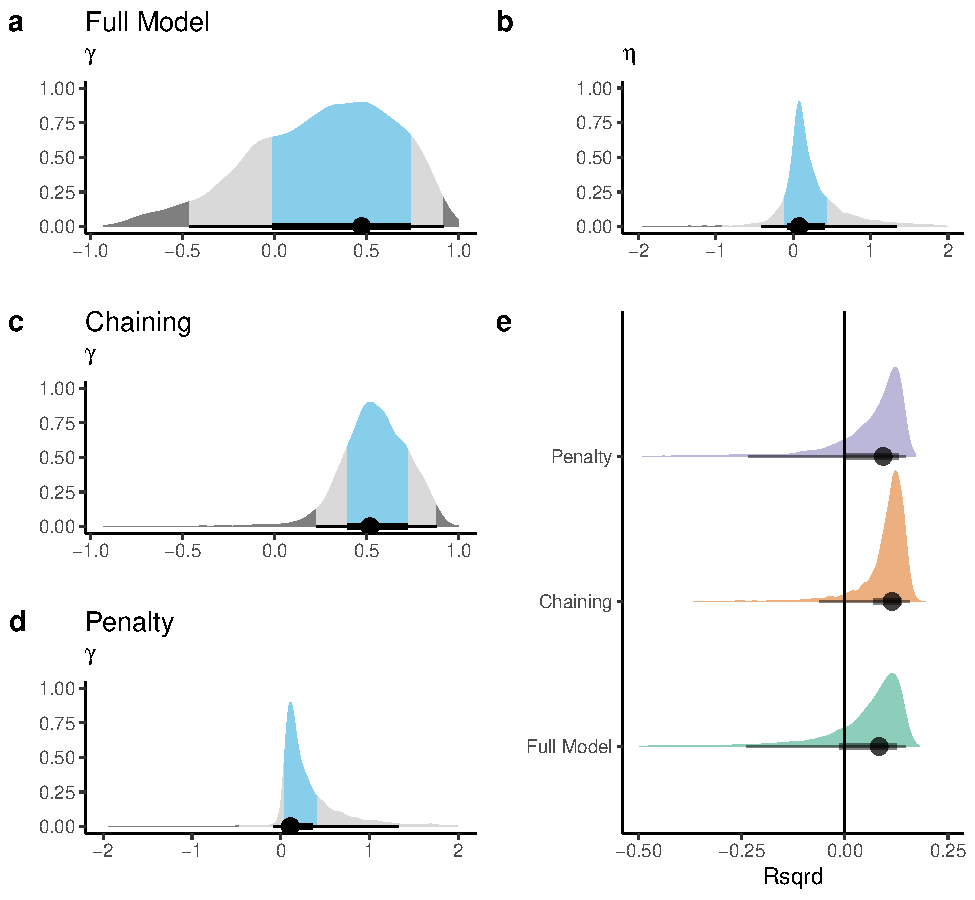
\includegraphics[width=1\linewidth]{manuscript_PLOS_files/figure-latex/post-1} \caption{Posterior distributions for parameter values $\gamma$ and $\eta$ for the three models (Full model, chaining only and penalty only). We show the kernel density estimates, below the mode (black dot) and the 65 (light blue shade) and 95\% (grey shade)  highest posterior density interval for the two parameters. On the top, panels a and b show posterior distributions for a full model, including chaining ($\gamma$) and penalty ($\eta$). Panel c, shows the $\gamma$ estimate from model with only chaining. Panel d shows the $\eta$ estimate from a model with only penalty. Panel e, shows a measure of fit for all models, namely the distribution of pseudo-$R^2$ obtained from sampling the posterior distribution of parameter values.}\label{fig:post}
\end{figure}

Estimation of parameter values for the three models (full model,
chaining and penalty), support chaining as the only mechanism cleaners
use to account for the future effects of their actions; and thus to
solve the ephemeral reward task. In the estimation of the parameter
values of the full model, which includes both chaining and penalty, the
bulk of the marginal posterior distribution of \(\eta\) which controls
the strength of penalty is around 0 (Fig. \ref{fig:post}). As for
\(\gamma\), controlling chaining, the 95\% confidence intervals also
includes zero, but the mode of the posterior is around 0.5 (Fig.
\ref{fig:post}, a). In the chaining model, where \(\eta\) is set to
zero, the distribution of \(\gamma\) shifted to higher values, zero is
no longer part of the 95\% credible interval of the parameter (Fig.
\ref{fig:post}, c). In contrast, when we look at the model with only
penalty, the posterior distribution of \(\eta\) is still centred around
zero (Fig. \ref{fig:post}, d). Thus, the analysis of the estimates of
individual parameter values in the three models only supports a strong
effect of chaining. Furthermore, the comparison of the models` fit
favours the chaining model. In panel e of figure \ref{fig:post} we show
the distribution of \(pseudo-R^2\) calculated using samples from the
posterior distributions shown before. Note, \(pseudo-R^2\) can have
negative values, which is when the log-likelihood of the model is lower
than that of a model that triggers neutral preferences. Even though the
peak of the three \(pseudo-R^2\) distributions were not very different,
the model with only chaining produced a distribution of \(pseudo-R^2\)
where more values were positive (to the right of the black line in Fig.
\ref{fig:post} f). This shows that accounting for variation in the
parameter estimates the model with chaining gives a better fit to the
data, despite having one parameter less than the full model. We have not
shown here the marginal posterior distributions of the scaling constant,
given that they do not bring biological insight. Their visualizations
can be found in the supplementary material (Fig. \ref{fig:scaConst}), as
well as the diagnostics of the MCMCs (Figs.
\ref{fig:diagnosticsfull},\ref{fig:diaggam},\ref{fig:diagNeg}).

\begin{figure}
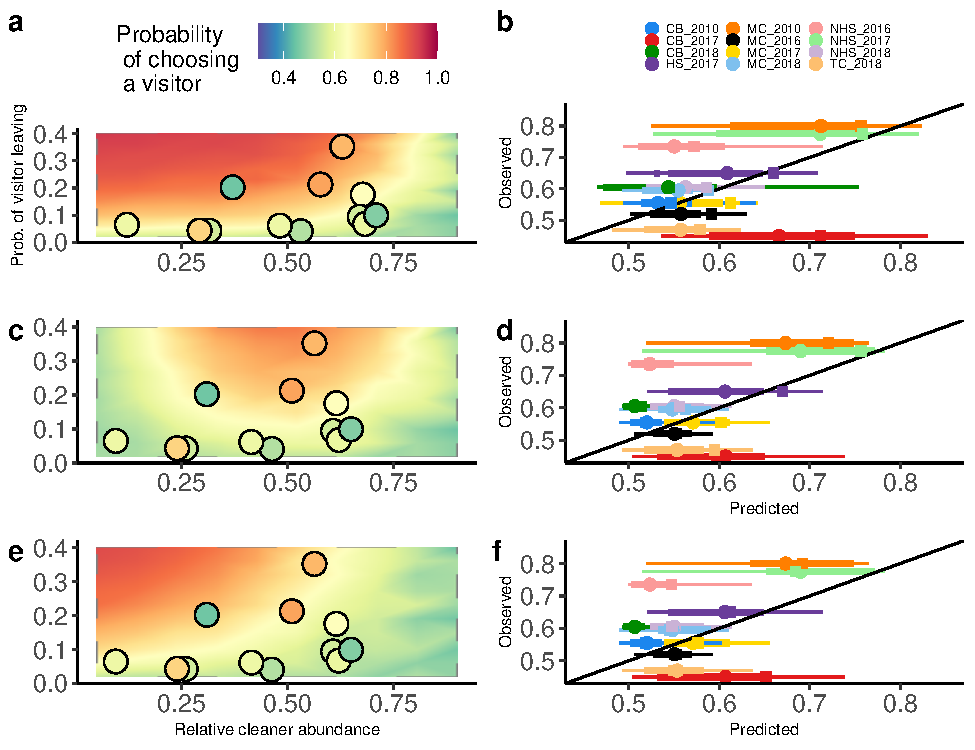
\includegraphics[width=1\linewidth]{manuscript_PLOS_files/figure-latex/pred-1} \caption{Observed and predicted probability of choosing a visitor. Left-hand side panel: colour contour shows the prediction from the learning model using the mode of the posterior distributions of parameters recovered by the statistical analysis. Dots show the frequency of visitor choices for the 12 reef sites, as well as the corresponding relative cleaner fish abundance (x axis) and frequency of visitors clients leaving the cleaning station (y axis). Right-hand side panels: Variation of the predicted probabilities  of choosing a visitor over a resident and their observed values for 12 locations. Circles show the mean prediction for each location from 100 samples taken from the posterior distribution. Thick and thin bars show the 66 and 95\% credible interval, respectively, taken from those posterior samples. Squares show the predictions used for the panel on the right-hand side. Colour coding denotes different reef site/year of the data collection (see Empirical data section). The black line corresponds to a perfect match between observed and predicted probabilities. Upper panels (a and b) show predictions from a model including chaining and penalty; middle panels (c and d) from a  model with only chaining; lower panels (e and f) from a model with penalty only.}\label{fig:pred}
\end{figure}

The main reason for chaining and penalty to give different predictions
is the way that cleaner fish relative abundance influences the
preference for the visitor clients. Visitor leaving probability has a
similar positive effect on the probability of choosing the visitor
clients on all three models, they all predict an increase preference for
visitors as the visitor probability increases (Fig. \ref{fig:pred}). In
contrast, cleaner fish relative abundance has a different effect in the
model with only chaining, compared to the other two models, full model
and penalty. In the model with only chaining, only intermediate cleaner
fish abundance triggers a preference for the visitor clients (Fig.
\ref{fig:pred} c). In both models with penalty, both intermediate and
low cleaner abundance triggered a preference for the visitor (Fig.
\ref{fig:pred} a,e). Note, however, we calculated preferences shown in
figure \ref{fig:pred} left panels by using only the mode of the
posterior distributions, and by holding constant the balance between
resident and visitors´ abundances. Panels on the right, show how close
predictions are from the observed data, allowing the balance between
client types to vary and using a set of samples from the posterior
distribution.

\hypertarget{discussion}{%
\subsection{Discussion}\label{discussion}}

In this study, our main aim was to unravel which of two potential
cognitive mechanisms, chaining of events, penalty, or their combination,
best explains wild-caught cleaner fish performance in the ephemeral
reward task, while accounting for their ecological conditions. To
evaluate the merits of each of these two mechanisms separately and
combined, we considered cleaner fish performance in the lab test to have
its origin from the rule these fish applied in their natural
environment. That is, individuals that solved the task already had a
preference for visitors clients and generalized this rule to the lab
conditions once being familiar with the task.

While all three models captured well the positive relationship between
visitor leaving behaviour and cleaner fish performance in the market
task {[}29{]}, only the chaining mechanism predicted that cleaner fish
performance in the task should be low in habitats with low
cleaner-to-client ratios, regardless of the visitor leaving probability.
In contrast, models including negative reward predicted the highest
performance in the ephemeral reward task when relative cleaner fish
abundance is low, particularly together with a high probability of
visitor leaving (Fig. \ref{fig:pred}). Low relative cleaner fish
abundances mean the market has an excess of demand for cleaning
services. In the models, this translates to a cleaning station that is
frequently full. Thus, when a visitor leaves, it is likely that the
cleaner fish will have access to another client in the next step.
Therefore, there will not be much difference in future reward between
choosing a visitor and a resident, and cleaners will not develop a
preference for the visitor in these conditions. On the other hand, the
effect of negative reward on cleaner fish preference is the opposite, as
in a busy cleaning station, to that of chaining. cleaner fish will get
more often the resident-visitor state and will develop a preference for
the visitor faster. At high cleaner fish abundances, the
resident-visitor state becomes so rare that neither mechanism is very
efficient at generating a preference for visitors. When facing the
resident-visitor choice, it is still best to choose the visitor;
however, the learning machinery will not be able to develop this
preference efficiently. Overall, the models suggest that chaining is the
cognitive mechanism that allows cleaner fish to adaptively adjust to
their biological market ecological conditions.

Previous research showed that cleaner fish living at high population
densities and giving service priority to the visitor plate in the
ephemeral reward task, as well as cleaner fish living at low densities
but denying service priority to the visitor plate possess larger
forebrains; a key teleost brain region associated with behavioural
flexibility and social intelligence. Those failing to show optimized
decision-rules given their local ecological conditions had relatively
smaller forebrains {[}30{]}. Triki \emph{et al.} refer to the former as
socially competent cleaner fish, while the second group as socially
incompetent cleaner fish. Social competence is the ability to optimise
social behaviour to the available social information {[}34--36{]}. Our
analyses yielded no evidence that the difference in social competence
with respect to the local ecological conditions and associated brain
morphology, found by Triki \emph{et al} {[}30{]}, is due to the
mechanism used to incorporate future consequences. It is conceivable
that high performing individuals from low population densities reef
sites use negative reinforcement instead of chaining, but in that case,
negative reinforcement should have explained at least part of the data.
Configurational learning or chunking {[}37,38{]}, the second component
necessary to solve the ephemeral reward task {[}22{]}, was not varied in
the models we analysed here. However, while chunking tendencies should
vary to allow individuals to adapt to their local conditions
{[}21,39{]}, systematic differences in individual chunking tendencies
would not explain how socially competent decisions vary as a function of
relative abundance. Therefore, it remains currently unclear what
cell-demanding mechanisms may cause variation in social competence that
translates into site-specific variation in performance in the ephemeral
reward task.

Our models are inspired by the general processes of associative learning
where short term rewards are translated into decision making; thus, it
ignores alternative channels of information that could be relevant in
market-like situations. For example, the model does not investigate
whether cleaner fish actually assess the frequency of client visits or a
mean frequency of visitors leaving. The updating learning mechanism for
the development of preferences works on a trial-by-trial basis. In the
model, cleaner fish do not need to assess the actual state of the
market, \emph{i.e.} their abundance, the abundance of residents and
visitors, and client visitation rate as an indicator of demand. They
only need to assess the short-term consequences of their own decisions
on food intake and chain them. Also, for the sake of simplicity, the
model ignores the process by which cleaner fish discriminate residents
and visitor clients. A model that accounts for this discrimination
probably would involve the development of preferences for morphological
or behavioural features that are statistically associated with visitors
or residents. For example, visitors are on average larger than residents
in body size {[}11{]}, and contrary to residents, they are less likely
to chase a cleaner fish that fails to cooperate and instead cheats its
client by taking a bite of mucus {[}12{]}. Given these associations,
chaining might produce the decision-rule ``choose the larger client
and/or the less aggressive client,'' which is not a useful rule in the
standard ephemeral reward task.

In conclusion, our study shows that variation in cognitive performance
as a function of the local ecological conditions may set the stage for
the use of mechanistic modelling to identify the cognitive processes
underlying learning in animals. The combination overcomes the
limitations of the general philosophy in animal cognition to apply the
logic of Lloyd Morgen's canon (Occam's razor). Cognitive experiments
with the aim of excluding basic reinforcement learning as a potential
explanation (operant and/or classical conditioning) of performance often
employ one trial experiments requiring animals to solve the task on the
first possible occasion. For example, any theory of mind task needs to
be solved in the first trial in order to exclude fast conditioning
{[}3{]}. Similarly, subjects need to solve a social learning task on the
first trial to accept imitation as a mechanism over stimulus/local
enhancement. Such strict conditions are virtually never met. For
example, potato washing by Japanese macaques, an iconic example of
social learning, took several years to spread within the group {[}40{]},
meaning that any learner had been repeatedly exposed to demonstrations
before acquisition. Importantly, Galef {[}41{]} refuted imitation as a
mechanism not simply because of the repeated exposure but because a
(rather qualitative) analysis of the spread of potato washing across
individuals did not follow the prediction based on imitation learning
(see also {[}42{]}). In our case, the number of trials it took cleaners
to learn the solution to the ephemeral rewards task would never allow
excluding an important role of penalty based on the data alone. However,
fitting model predictions to our comprehensive empirical data set
revealed that a more complex mechanism, estimation of future reward,
fits the data better.

\newpage

\hypertarget{supplementary-material}{%
\section{Supplementary material}\label{supplementary-material}}

\beginsupplement

\begin{figure}
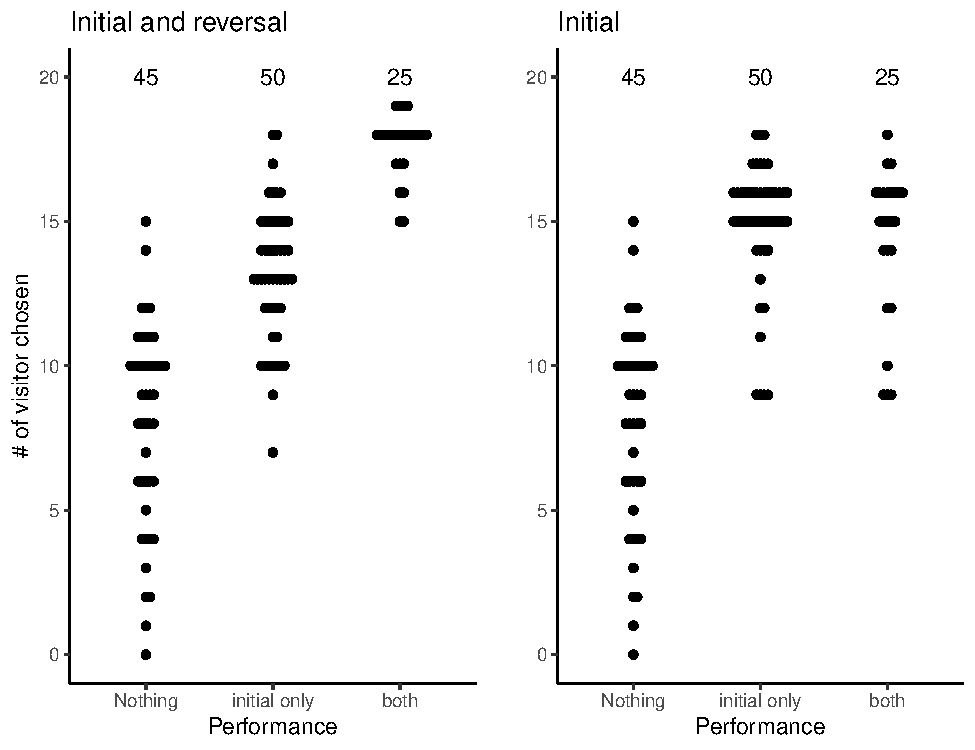
\includegraphics[width=1\linewidth]{manuscript_PLOS_files/figure-latex/rawdata-1} \caption{Relation between the response variable used in this study and the criteria used in previous studies to assess performance in the ephemeral reward task. In the x axis, we classified the performance of cleaner fish according to whether they developed a preference for the visitor in the initial round, in the initial and reversal, or none of them. In the y axis, we add the choices of two experimental sessions: panel on the left uses one session from the initial round and one from the reversal round when possible (as described in the main text); panel on the right uses two sessions from the initial round for all fish.}\label{fig:rawdata}
\end{figure}

\begin{figure}[H]
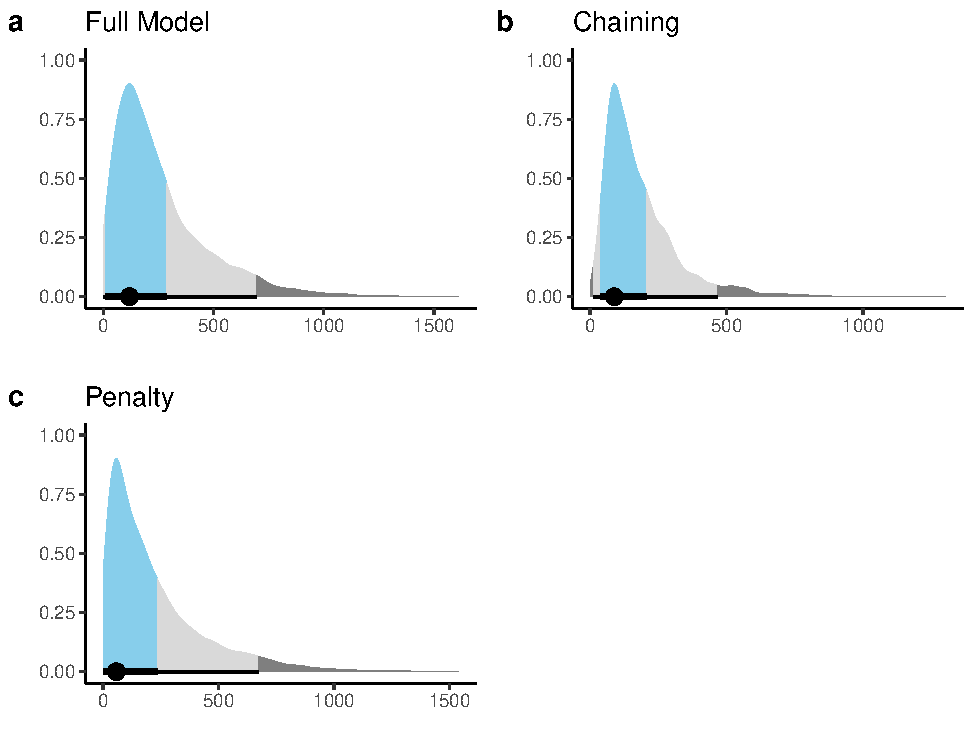
\includegraphics[width=0.95\linewidth,]{manuscript_PLOS_files/figure-latex/scaConst-1} \caption{Posterior distributions for scaling constant for the three models (Full model, chaining only and penalty only). We show the kernel density estimates, below the mode (black dot) and the 65\% (light blue shade) and 95\% (grey shade)  highest posterior density interval. On the top, panel a shows the posterior distribution from the full model; panel b from the model with only chaining; and panel c from a model with only penalty.}\label{fig:scaConst}
\end{figure}

\begin{figure}
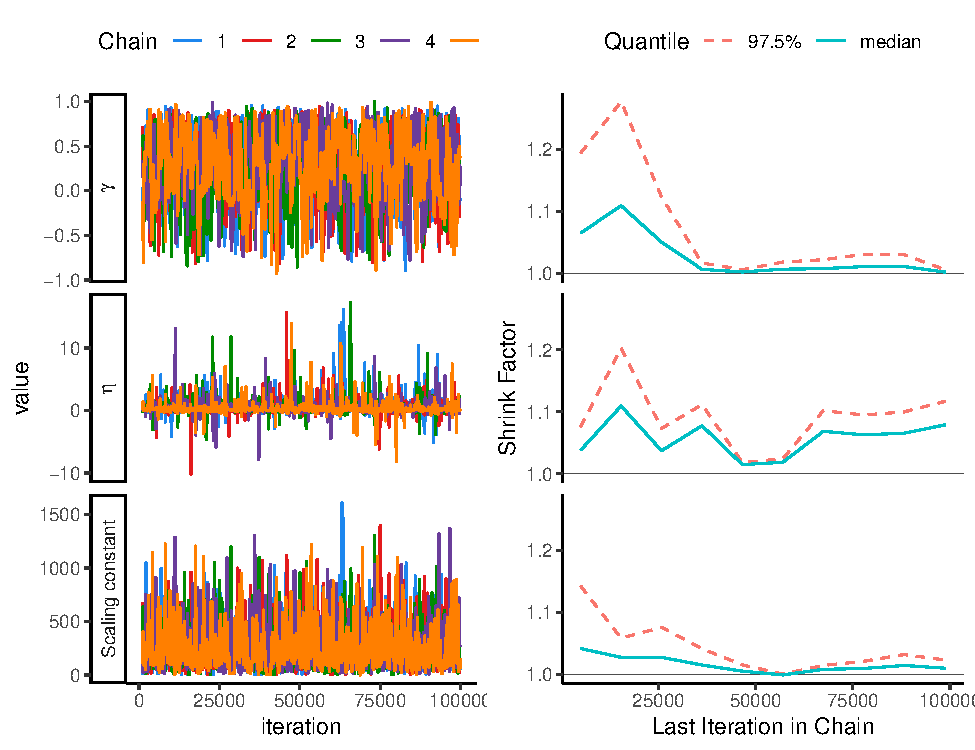
\includegraphics[width=1\linewidth]{manuscript_PLOS_files/figure-latex/diagnosticsfull-1} \caption{MCMC convergence diagnostics for the full model. On the left trace-plots, on the right changes along the chain of the Gelman and Rubin shrink factor.}\label{fig:diagnosticsfull}
\end{figure}

\begin{figure}
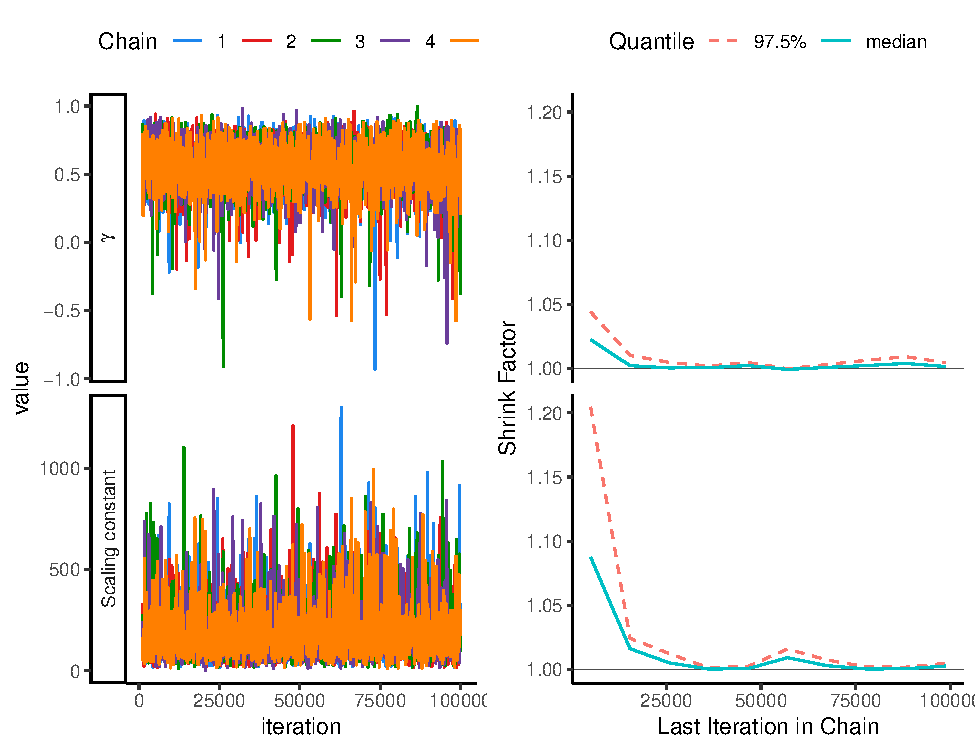
\includegraphics[width=1\linewidth]{manuscript_PLOS_files/figure-latex/diaggam-1} \caption{MCMC convergence diagnostics for the chaining model. On the left trace-plots, on the right changes along the chain of the Gelman and Rubin shrink factor }\label{fig:diaggam}
\end{figure}

\begin{figure}
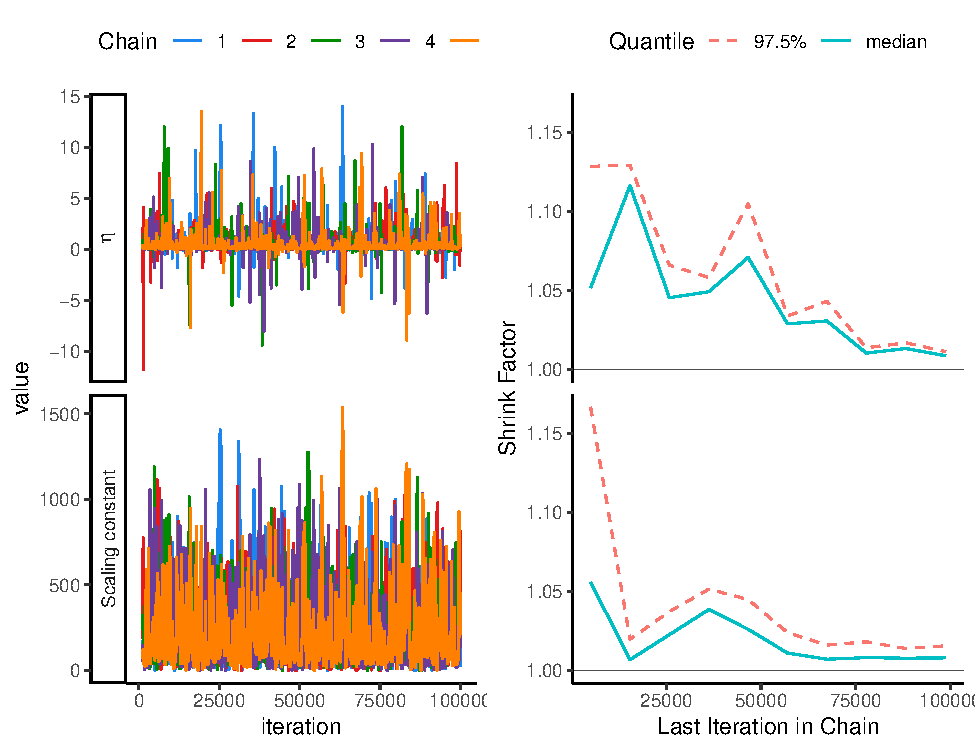
\includegraphics[width=1\linewidth]{manuscript_PLOS_files/figure-latex/diagNeg-1} \caption{MCMC convergence diagnostics for the penalty model. On the left trace-plots, on the right changes along the chain of the Gelman and Rubin shrink factor}\label{fig:diagNeg}
\end{figure}

\begin{longtable}[]{@{}rc@{}}
\caption{\label{tab:param} Parameter values with which the model was run
in the MCMC. \(\sigma\) refers to the amplitude of the perturbation
kernel with the subscript indicating the associated parameter. New
values were taken from a uniform distribution. \(\alpha\) refers to the
learning rate.}\tabularnewline
\toprule
Parameter & Value \\
\midrule
\endfirsthead
\toprule
Parameter & Value \\
\midrule
\endhead
Learning rounds & 10000 \\
Reward value & 1 \\
\(\alpha\) & 0.05 \\
\(\sigma_{\gamma}\) & 0.3 \\
\(\sigma_{\eta}\) & 4 \\
\(\sigma_{Sca.Const.}\) & 300 \\
Number of chains & 5 \\
Chain length & \(1^5\) \\
\bottomrule
\end{longtable}

\hypertarget{references}{%
\section*{References}\label{references}}
\addcontentsline{toc}{section}{References}

\hypertarget{refs}{}
\begin{CSLReferences}{0}{0}
\leavevmode\vadjust pre{\hypertarget{ref-dally_Foodcaching_2006}{}}%
\CSLLeftMargin{1. }
\CSLRightInline{Dally JM, Emery NJ, Clayton NS. Food-caching western
scrub-jays keep track of who was watching when. Science (New York, NY).
2006;312: 1662--1665.
doi:\href{https://doi.org/10.1126/science.1126539}{10.1126/science.1126539}}

\leavevmode\vadjust pre{\hypertarget{ref-suddendorf_Evolution_2007}{}}%
\CSLLeftMargin{2. }
\CSLRightInline{Suddendorf T, Corballis MC. The evolution of foresight:
{What} is mental time travel, and is it unique to humans? The Behavioral
and Brain Sciences. 2007;30: 299-313; discussion 313-351.
doi:\href{https://doi.org/10.1017/S0140525X07001975}{10.1017/S0140525X07001975}}

\leavevmode\vadjust pre{\hypertarget{ref-heyes_Theory_1998}{}}%
\CSLLeftMargin{3. }
\CSLRightInline{Heyes CM. Theory of mind in nonhuman primates.
Behavioral and Brain Sciences. 1998;21: 101--114.
doi:\href{https://doi.org/10.1017/S0140525X98000703}{10.1017/S0140525X98000703}}

\leavevmode\vadjust pre{\hypertarget{ref-noe_Biological_1995}{}}%
\CSLLeftMargin{4. }
\CSLRightInline{Noë R, Hammerstein P. Biological markets. Trends in
Ecology \& Evolution. 1995;10: 336--339.
doi:\href{https://doi.org/10.1016/S0169-5347(00)89123-5}{10.1016/S0169-5347(00)89123-5}}

\leavevmode\vadjust pre{\hypertarget{ref-axen_Signalling_1996}{}}%
\CSLLeftMargin{5. }
\CSLRightInline{Axén AH, Leimar O, Hoffman V. Signalling in a
mutualistic interaction. Animal Behaviour. 1996;52: 321--333.
doi:\href{https://doi.org/10.1006/anbe.1996.0178}{10.1006/anbe.1996.0178}}

\leavevmode\vadjust pre{\hypertarget{ref-waldie_LongTerm_2011}{}}%
\CSLLeftMargin{6. }
\CSLRightInline{Waldie PA, Blomberg SP, Cheney KL, Goldizen AW, Grutter
AS. Long-{Term} {Effects} of the {Cleaner} {Fish} {Labroides} dimidiatus
on {Coral} {Reef} {Fish} {Communities}. PLOS ONE. 2011;6: e21201.
doi:\href{https://doi.org/10.1371/journal.pone.0021201}{10.1371/journal.pone.0021201}}

\leavevmode\vadjust pre{\hypertarget{ref-ros_Does_2011}{}}%
\CSLLeftMargin{7. }
\CSLRightInline{Ros AFH, Lusa J, Meyer M, Soares M, Oliveira RF,
Brossard M, et al. Does access to the bluestreak cleaner wrasse
{Labroides} dimidiatus affect indicators of stress and health in
resident reef fishes in the {Red} {Sea}? Hormones and Behavior. 2011;59:
151--158.
doi:\href{https://doi.org/10.1016/j.yhbeh.2010.11.006}{10.1016/j.yhbeh.2010.11.006}}

\leavevmode\vadjust pre{\hypertarget{ref-triki_Effects_2016}{}}%
\CSLLeftMargin{8. }
\CSLRightInline{Triki Z, Grutter AS, Bshary R, Ros AFH. Effects of
short-term exposure to ectoparasites on fish cortisol and hematocrit
levels. Marine Biology. 2016;163: 187.
doi:\href{https://doi.org/10.1007/s00227-016-2959-y}{10.1007/s00227-016-2959-y}}

\leavevmode\vadjust pre{\hypertarget{ref-demaire_Reduced_2020}{}}%
\CSLLeftMargin{9. }
\CSLRightInline{Demairé C, Triki Z, Binning SA, Glauser G, Roche DG,
Bshary R. Reduced access to cleaner fish negatively impacts the
physiological state of two resident reef fishes. Marine Biology.
2020;167: 48.
doi:\href{https://doi.org/10.1007/s00227-020-3658-2}{10.1007/s00227-020-3658-2}}

\leavevmode\vadjust pre{\hypertarget{ref-bshary_Choosy_2002}{}}%
\CSLLeftMargin{10. }
\CSLRightInline{Bshary R, Schäffer D. Choosy reef fish select cleaner
fish that provide high-quality service. Animal Behaviour. 2002;63:
557--564.
doi:\href{https://doi.org/10.1006/anbe.2001.1923}{10.1006/anbe.2001.1923}}

\leavevmode\vadjust pre{\hypertarget{ref-bshary_Cleaner_2001}{}}%
\CSLLeftMargin{11. }
\CSLRightInline{Bshary R. The cleaner fish market. In: Van Hooff JARAM,
Hammerstein P, Noë R, editors. Economics in {Nature}: {Social}
{Dilemmas}, {Mate} {Choice} and {Biological} {Markets}. Cambridge:
Cambridge University Press; 2001. pp. 146--172.
doi:\href{https://doi.org/10.1017/CBO9780511752421.010}{10.1017/CBO9780511752421.010}}

\leavevmode\vadjust pre{\hypertarget{ref-bshary_Asymmetric_2002}{}}%
\CSLLeftMargin{12. }
\CSLRightInline{Bshary R, Grutter AS. Asymmetric cheating opportunities
and partner control in a cleaner fish mutualism. Animal Behaviour.
2002;63: 547--555.
doi:\href{https://doi.org/10.1006/anbe.2001.1937}{10.1006/anbe.2001.1937}}

\leavevmode\vadjust pre{\hypertarget{ref-salwiczek_Adult_2012}{}}%
\CSLLeftMargin{13. }
\CSLRightInline{Salwiczek LH, Prétôt L, Demarta L, Proctor D, Essler J,
Pinto AI, et al. Adult {Cleaner} {Wrasse} {Outperform} {Capuchin}
{Monkeys}, {Chimpanzees} and {Orang}-utans in a {Complex} {Foraging}
{Task} {Derived} from {Cleaner} -- {Client} {Reef} {Fish} {Cooperation}.
PLOS ONE. 2012;7: e49068.
doi:\href{https://doi.org/10.1371/journal.pone.0049068}{10.1371/journal.pone.0049068}}

\leavevmode\vadjust pre{\hypertarget{ref-zentall_Early_2017}{}}%
\CSLLeftMargin{14. }
\CSLRightInline{Zentall TR, Case JP, Berry JR. Early commitment
facilitates optimal choice by pigeons. Psychonomic Bulletin \& Review.
2017;24: 957--963.
doi:\href{https://doi.org/10.3758/s13423-016-1173-8}{10.3758/s13423-016-1173-8}}

\leavevmode\vadjust pre{\hypertarget{ref-pepperberg_Can_2014}{}}%
\CSLLeftMargin{15. }
\CSLRightInline{Pepperberg IM, Hartsfield LA. Can grey parrots
({Psittacus} erithacus) succeed on a "complex" foraging task failed by
nonhuman primates ({Pan} troglodytes, {Pongo} abelii, {Sapajus} apella)
but solved by wrasse fish ({Labroides} dimidiatus)? Journal of
Comparative Psychology (Washington, DC: 1983). 2014;128: 298--306.
doi:\href{https://doi.org/10.1037/a0036205}{10.1037/a0036205}}

\leavevmode\vadjust pre{\hypertarget{ref-shettleworth_Cognition_2009}{}}%
\CSLLeftMargin{16. }
\CSLRightInline{Shettleworth SJ. Cognition, {Evolution}, and {Behavior}.
2 edition. Oxford ; New York: Oxford University Press; 2009. }

\leavevmode\vadjust pre{\hypertarget{ref-wismer_Cuebased_2019}{}}%
\CSLLeftMargin{17. }
\CSLRightInline{Wismer S, Pinto AI, Triki Z, Grutter AS, Roche DG,
Bshary R. Cue-based decision rules of cleaner fish in a biological
market task. Animal Behaviour. 2019 {[}cited 30 Oct 2019{]}.
doi:\href{https://doi.org/10.1016/j.anbehav.2019.09.013}{10.1016/j.anbehav.2019.09.013}}

\leavevmode\vadjust pre{\hypertarget{ref-pretot_Comparative_2021}{}}%
\CSLLeftMargin{18. }
\CSLRightInline{Prétôt L, Mickelberg J, Carrigan J, Stoinski T, Bshary
R, Brosnan SF. Comparative performance of orangutans ({Pongo} spp.),
Gorillas ({Gorilla} gorilla gorilla), and drills ({Mandrillus}
leucophaeus), in an ephemeral foraging task. American Journal of
Primatology. 2021;83: e23212.
doi:\href{https://doi.org/10.1002/ajp.23212}{10.1002/ajp.23212}}

\leavevmode\vadjust pre{\hypertarget{ref-pretot_Comparing_2016}{}}%
\CSLLeftMargin{19. }
\CSLRightInline{Prétôt L, Bshary R, Brosnan SF. Comparing species
decisions in a dichotomous choice task: Adjusting task parameters
improves performance in monkeys. Animal Cognition. 2016;19: 819--834.
doi:\href{https://doi.org/10.1007/s10071-016-0981-6}{10.1007/s10071-016-0981-6}}

\leavevmode\vadjust pre{\hypertarget{ref-dubois_Model_2021}{}}%
\CSLLeftMargin{20. }
\CSLRightInline{Dubois T, Pasquaretta C, Barron AB, Gautrais J, Lihoreau
M. A model of resource partitioning between foraging bees based on
learning. PLOS Computational Biology. 2021;17: e1009260.
doi:\href{https://doi.org/10.1371/journal.pcbi.1009260}{10.1371/journal.pcbi.1009260}}

\leavevmode\vadjust pre{\hypertarget{ref-prat_Modelling_2022}{}}%
\CSLLeftMargin{21. }
\CSLRightInline{Prat Y, Bshary R, Lotem A. Modelling how cleaner fish
approach an ephemeral reward task demonstrates a role for ecologically
tuned chunking in the evolution of advanced cognition. PLOS Biology.
2022;20: e3001519.
doi:\href{https://doi.org/10.1371/journal.pbio.3001519}{10.1371/journal.pbio.3001519}}

\leavevmode\vadjust pre{\hypertarget{ref-quinones_Reinforcement_2019}{}}%
\CSLLeftMargin{22. }
\CSLRightInline{Quiñones AE, Leimar O, Lotem A, Bshary R. Reinforcement
{Learning} {Theory} {Reveals} the {Cognitive} {Requirements} for
{Solving} the {Cleaner} {Fish} {Market} {Task}. The American Naturalist.
2019; 000--000.
doi:\href{https://doi.org/10.1086/707519}{10.1086/707519}}

\leavevmode\vadjust pre{\hypertarget{ref-enquist_Power_2016}{}}%
\CSLLeftMargin{23. }
\CSLRightInline{Enquist M, Lind J, Ghirlanda S. The power of associative
learning and the ontogeny of optimal behaviour. Royal Society Open
Science. 2016;3: 160734.
doi:\href{https://doi.org/10.1098/rsos.160734}{10.1098/rsos.160734}}

\leavevmode\vadjust pre{\hypertarget{ref-sutton_Reinforcement_2018}{}}%
\CSLLeftMargin{24. }
\CSLRightInline{Sutton RS, Barto AG. Reinforcement {Learning}: {An}
{Introduction}. second edition edition. Bach F, editor. Cambridge, MA: A
Bradford Book; 2018. }

\leavevmode\vadjust pre{\hypertarget{ref-thorndike_Animal_1898}{}}%
\CSLLeftMargin{25. }
\CSLRightInline{Thorndike EL. Animal intelligence: {An} experimental
study of the associative processes in animals. The Psychological Review:
Monograph Supplements. 1898;2: i--109.
doi:\href{https://doi.org/10.1037/h0092987}{10.1037/h0092987}}

\leavevmode\vadjust pre{\hypertarget{ref-skinner_Behavior_1938}{}}%
\CSLLeftMargin{26. }
\CSLRightInline{Skinner BF. The behavior of organisms;: {An}
experimental analysis,. 1938. }

\leavevmode\vadjust pre{\hypertarget{ref-wismer_Variation_2014}{}}%
\CSLLeftMargin{27. }
\CSLRightInline{Wismer S, Pinto AI, Vail AL, Grutter AS, Bshary R.
Variation in {Cleaner} {Wrasse} {Cooperation} and {Cognition}:
{Influence} of the {Developmental} {Environment}? Ethology. 2014;120:
519--531.
doi:\href{https://doi.org/10.1111/eth.12223}{10.1111/eth.12223}}

\leavevmode\vadjust pre{\hypertarget{ref-triki_Decrease_2018}{}}%
\CSLLeftMargin{28. }
\CSLRightInline{Triki Z, Wismer S, Levorato E, Bshary R. A decrease in
the abundance and strategic sophistication of cleaner fish after
environmental perturbations. Global Change Biology. 2018;24: 481--489.
doi:\href{https://doi.org/10.1111/gcb.13943}{10.1111/gcb.13943}}

\leavevmode\vadjust pre{\hypertarget{ref-triki_Biological_2019}{}}%
\CSLLeftMargin{29. }
\CSLRightInline{Triki Z, Wismer S, Rey O, Ann Binning S, Levorato E,
Bshary R. Biological market effects predict cleaner fish strategic
sophistication. Behavioral Ecology. 2019;30: 1548--1557.
doi:\href{https://doi.org/10.1093/beheco/arz111}{10.1093/beheco/arz111}}

\leavevmode\vadjust pre{\hypertarget{ref-triki_Brain_2020}{}}%
\CSLLeftMargin{30. }
\CSLRightInline{Triki Z, Emery Y, Teles MC, Oliveira RF, Bshary R. Brain
morphology predicts social intelligence in wild cleaner fish. Nature
Communications. 2020;11: 6423.
doi:\href{https://doi.org/10.1038/s41467-020-20130-2}{10.1038/s41467-020-20130-2}}

\leavevmode\vadjust pre{\hypertarget{ref-rescorla_Theory_1972}{}}%
\CSLLeftMargin{31. }
\CSLRightInline{Rescorla RA, Wagner ARA. A theory of {Pavlovian}
conditioning: Variations in the effectiveness of reinforcement and
non-reinforcement. In: Black AH, Prokasy WF, editors. Classical
conditioning {II}: Current research and theory. New York:
Appleton-Century-Crofts; 1972. }

\leavevmode\vadjust pre{\hypertarget{ref-rcoreteam_Language_2021}{}}%
\CSLLeftMargin{32. }
\CSLRightInline{R Core Team. R: {A} language and environment for
statistical computing. Vienna, Austria; 2021. Available:
\url{https://www.R-project.org/}}

\leavevmode\vadjust pre{\hypertarget{ref-mcfadden_Conditional_1974}{}}%
\CSLLeftMargin{33. }
\CSLRightInline{McFadden D. Conditional logit analysis of qualitative
choice behavior. Frontiers in econometrics. 1974. }

\leavevmode\vadjust pre{\hypertarget{ref-taborsky_Social_2012}{}}%
\CSLLeftMargin{34. }
\CSLRightInline{Taborsky B, Oliveira RF. Social competence: An
evolutionary approach. Trends in Ecology \& Evolution. 2012;27:
679--688.
doi:\href{https://doi.org/10.1016/j.tree.2012.09.003}{10.1016/j.tree.2012.09.003}}

\leavevmode\vadjust pre{\hypertarget{ref-bshary_Cooperation_2015}{}}%
\CSLLeftMargin{35. }
\CSLRightInline{Bshary R, Oliveira RF. Cooperation in animals: Toward a
game theory within the framework of social competence. Current Opinion
in Behavioral Sciences. 2015;3: 31--37.
doi:\href{https://doi.org/10.1016/j.cobeha.2015.01.008}{10.1016/j.cobeha.2015.01.008}}

\leavevmode\vadjust pre{\hypertarget{ref-varela_Correlated_2020}{}}%
\CSLLeftMargin{36. }
\CSLRightInline{Varela SAM, Teles MC, Oliveira RF. The correlated
evolution of social competence and social cognition. Functional Ecology.
2020;34: 332--343.
doi:\href{https://doi.org/10.1111/1365-2435.13416}{10.1111/1365-2435.13416}}

\leavevmode\vadjust pre{\hypertarget{ref-sutherland_Configural_1989}{}}%
\CSLLeftMargin{37. }
\CSLRightInline{Sutherland RJ, Rudy JW. Configural association theory:
{The} role of the hippocampal formation in learning, memory, and
amnesia. Psychobiology. 1989;17: 129--144.
doi:\href{https://doi.org/10.3758/BF03337828}{10.3758/BF03337828}}

\leavevmode\vadjust pre{\hypertarget{ref-miller_Magical_1956}{}}%
\CSLLeftMargin{38. }
\CSLRightInline{Miller GA. The magical number seven, plus or minus two:
{Some} limits on our capacity for processing information. Psychological
review. 1956;63: 81. }

\leavevmode\vadjust pre{\hypertarget{ref-kolodny_Evolution_2014}{}}%
\CSLLeftMargin{39. }
\CSLRightInline{Kolodny O, Edelman S, Lotem A. The evolution of
continuous learning of the structure of the environment. Journal of The
Royal Society Interface. 2014;11: 20131091--20131091.
doi:\href{https://doi.org/10.1098/rsif.2013.1091}{10.1098/rsif.2013.1091}}

\leavevmode\vadjust pre{\hypertarget{ref-kawamura_Process_1959}{}}%
\CSLLeftMargin{40. }
\CSLRightInline{Kawamura S. The process of sub-culture propagation among
{Japanese} macaques. Primates. 1959;2: 43--60.
doi:\href{https://doi.org/10.1007/BF01666110}{10.1007/BF01666110}}

\leavevmode\vadjust pre{\hypertarget{ref-galef_Question_1992}{}}%
\CSLLeftMargin{41. }
\CSLRightInline{Galef BG. The question of animal culture. Human Nature.
1992;3: 157--178.
doi:\href{https://doi.org/10.1007/BF02692251}{10.1007/BF02692251}}

\leavevmode\vadjust pre{\hypertarget{ref-hirata_SweetPotato_2001}{}}%
\CSLLeftMargin{42. }
\CSLRightInline{Hirata S, Watanabe K, Masao K. {``{Sweet}-{Potato}
{Washing}''} {Revisited}. In: Matsuzawa T, editor. Primate {Origins} of
{Human} {Cognition} and {Behavior}. Tokyo: Springer Japan; 2001. pp.
487--508.
doi:\href{https://doi.org/10.1007/978-4-431-09423-4_24}{10.1007/978-4-431-09423-4\_24}}

\end{CSLReferences}

\nolinenumbers



\end{document}
